\chapter{Evaluations}

\newcommand{\round}[1]{\DTLround{#1}{#1}{4}#1}

\section{Evaluation setup}

define evaluations and justify
discussion for each section

\subsection{Data completeness}

\begin{table}[H]
    \begin{tabular}{|c|c|}
    \hline
    Total number of public personal profiles & 13014 \\ \hline
    Total number of company profiles         & 24778 \\ \hline
    Total number of skills                   & 15917 \\ \hline
    \end{tabular}
\end{table}

\subsubsection{Public personal profile completeness}

\begin{table}[H]
    \begin{tabular}{|c|c|c|}
    \hline
    ~                                                             & Number & Percentage(of personal profiles) \\ \hline
    Profiles that have work experiences                           & 11501  & 88.4\%                             \\ \hline
    Profiles that have education                                  & 9913   & 77\%                               \\ \hline
    Profiles that have skills                                     & 10511  & 80\%                               \\ \hline
    Profiles that have city infomation & 10158  & 78\%                               \\ \hline
    Profiles that have academic degree information                & 5230   & 40.2\%                             \\ \hline
    Profiles that have college major information                  & 7825   & 60.1\%                             \\ \hline
    \end{tabular}
\end{table}

\subsubsection{Company profile completeness}
\begin{table}[H]
    \begin{tabular}{|c|c|c|}
    \hline
    ~                                            & Number & Percentage(of company profiles) \\ \hline
    Company profiles that have industry type     & 11868  & 47.9\%                             \\ \hline
    Company profiles that have organisation type & 11351  & 45.8\%                             \\ \hline
    Company profiles that have company size info & 11343  & 45.8\%                             \\ \hline
    \end{tabular}
\end{table}

\subsubsection{Data linkage}

\begin{table}[H]
    \begin{tabular}{|c|c|}
    \hline
    Total number of objects & 160251 \\ \hline
    Total number of links   & 415916 \\ \hline
    Linkage                 & 2.595  \\ \hline
    \end{tabular}
\end{table}

\subsection{Metadata quality}

\begin{table}[H]
	\centering
	\DTLloaddb[keys={user,precision,recall,fmeasure}]{citycsv}{csvs/city.csv}
	\caption{Precision, recall and f-measure scores for city information}
	\begin{tabular}{|c|c|c|c|}
	\toprule \hline 
	\bfseries User & \bfseries Precision & \bfseries Recall & \bfseries F-Measure
	\DTLforeach{citycsv}{\user=user, \precision=precision, \recall=recall, \fmeasure=fmeasure}{%
	\ifthenelse{\value{DTLrowi}=1}{\tabularnewline \hline}{\tabularnewline}
	\user & \round{\precision} & \round{\recall} & \round{\fmeasure}} \\
	\hline \bottomrule
	\end{tabular}
	\label{tab:cityResult}
\end{table}

\begin{table}[H]
	\centering
	\DTLloaddb[keys={user,precision,recall,fmeasure}]{companycsv}{csvs/company.csv}
	\caption{Precision, recall and f-measure scores for company information}
	\begin{tabular}{|c|c|c|c|}
	\toprule \hline 
	\bfseries User & \bfseries Precision & \bfseries Recall & \bfseries F-Measure
	\DTLforeach{companycsv}{\user=user, \precision=precision, \recall=recall, \fmeasure=fmeasure}{%
	\ifthenelse{\value{DTLrowi}=1}{\tabularnewline \hline}{\tabularnewline}
	\user & \round{\precision} & \round{\recall} & \round{\fmeasure}} \\
	\hline \bottomrule
	\end{tabular}
	\label{tab:companyResult}
\end{table}

\begin{table}[H]
	\centering
	\DTLloaddb[keys={user,precision,recall,fmeasure}]{jobtitlecsv}{csvs/job_title.csv}
	\caption{Precision, recall and f-measure scores for job title information}
	\begin{tabular}{|c|c|c|c|}
	\toprule \hline 
	\bfseries User & \bfseries Precision & \bfseries Recall & \bfseries F-Measure
	\DTLforeach{jobtitlecsv}{\user=user, \precision=precision, \recall=recall, \fmeasure=fmeasure}{%
	\ifthenelse{\value{DTLrowi}=1}{\tabularnewline \hline}{\tabularnewline}
	\user & \round{\precision} & \round{\recall} & \round{\fmeasure}} \\
	\hline \bottomrule
	\end{tabular}
	\label{tab:jobtitleResult}
\end{table}

\begin{table}[H]
	\centering
	\DTLloaddb[keys={user,precision,recall,fmeasure}]{experiencefromcsv}{csvs/experience_from.csv}
	\caption{Precision, recall and f-measure scores for experience start date information}
	\begin{tabular}{|c|c|c|c|}
	\toprule \hline 
	\bfseries User & \bfseries Precision & \bfseries Recall & \bfseries F-Measure
	\DTLforeach{experiencefromcsv}{\user=user, \precision=precision, \recall=recall, \fmeasure=fmeasure}{%
	\ifthenelse{\value{DTLrowi}=1}{\tabularnewline \hline}{\tabularnewline}
	\user & \round{\precision} & \round{\recall} & \round{\fmeasure}} \\
	\hline \bottomrule
	\end{tabular}
	\label{tab:experiencefromResult}
\end{table}

\begin{table}[H]
	\centering
	\DTLloaddb[keys={user,precision,recall,fmeasure}]{experiencetocsv}{csvs/experience_to.csv}
	\caption{Precision, recall and f-measure scores for experience end date information}
	\begin{tabular}{|c|c|c|c|}
	\toprule \hline 
	\bfseries User & \bfseries Precision & \bfseries Recall & \bfseries F-Measure
	\DTLforeach{experiencetocsv}{\user=user, \precision=precision, \recall=recall, \fmeasure=fmeasure}{%
	\ifthenelse{\value{DTLrowi}=1}{\tabularnewline \hline}{\tabularnewline}
	\user & \round{\precision} & \round{\recall} & \round{\fmeasure}} \\
	\hline \bottomrule
	\end{tabular}
	\label{tab:experiencetoResult}
\end{table}

\begin{table}[H]
	\centering
	\DTLloaddb[keys={user,precision,recall,fmeasure}]{collegecsv}{csvs/college.csv}
	\caption{Precision, recall and f-measure scores for college information}
	\begin{tabular}{|c|c|c|c|}
	\toprule \hline 
	\bfseries User & \bfseries Precision & \bfseries Recall & \bfseries F-Measure
	\DTLforeach{collegecsv}{\user=user, \precision=precision, \recall=recall, \fmeasure=fmeasure}{%
	\ifthenelse{\value{DTLrowi}=1}{\tabularnewline \hline}{\tabularnewline}
	\user & \round{\precision} & \round{\recall} & \round{\fmeasure}} \\
	\hline \bottomrule
	\end{tabular}
	\label{tab:collegeResult}
\end{table}

\begin{table}[H]
	\centering
	\DTLloaddb[keys={user,precision,recall,fmeasure}]{majorcsv}{csvs/major.csv}
	\caption{Precision, recall and f-measure scores for major information}
	\begin{tabular}{|c|c|c|c|}
	\toprule \hline 
	\bfseries User & \bfseries Precision & \bfseries Recall & \bfseries F-Measure
	\DTLforeach{majorcsv}{\user=user, \precision=precision, \recall=recall, \fmeasure=fmeasure}{%
	\ifthenelse{\value{DTLrowi}=1}{\tabularnewline \hline}{\tabularnewline}
	\user & \round{\precision} & \round{\recall} & \round{\fmeasure}} \\
	\hline \bottomrule
	\end{tabular}
	\label{tab:majorResult}
\end{table}

\begin{table}[H]
	\centering
	\DTLloaddb[keys={user,precision,recall,fmeasure}]{degreecsv}{csvs/degree.csv}
	\caption{Precision, recall and f-measure scores for degree information}
	\begin{tabular}{|c|c|c|c|}
	\toprule \hline 
	\bfseries User & \bfseries Precision & \bfseries Recall & \bfseries F-Measure
	\DTLforeach{degreecsv}{\user=user, \precision=precision, \recall=recall, \fmeasure=fmeasure}{%
	\ifthenelse{\value{DTLrowi}=1}{\tabularnewline \hline}{\tabularnewline}
	\user & \round{\precision} & \round{\recall} & \round{\fmeasure}} \\
	\hline \bottomrule
	\end{tabular}
	\label{tab:degreeResult}
\end{table}

\begin{table}[H]
	\centering
	\DTLloaddb[keys={user,precision,recall,fmeasure}]{educationfromcsv}{csvs/education_from.csv}
	\caption{Precision, recall and f-measure scores for education start date information}
	\begin{tabular}{|c|c|c|c|}
	\toprule \hline 
	\bfseries User & \bfseries Precision & \bfseries Recall & \bfseries F-Measure
	\DTLforeach{educationfromcsv}{\user=user, \precision=precision, \recall=recall, \fmeasure=fmeasure}{%
	\ifthenelse{\value{DTLrowi}=1}{\tabularnewline \hline}{\tabularnewline}
	\user & \round{\precision} & \round{\recall} & \round{\fmeasure}} \\
	\hline \bottomrule
	\end{tabular}
	\label{tab:educationfromResult}
\end{table}

\begin{table}[H]
	\centering
	\DTLloaddb[keys={user,precision,recall,fmeasure}]{educationtocsv}{csvs/education_to.csv}
	\caption{Precision, recall and f-measure scores for education end date information}
	\begin{tabular}{|c|c|c|c|}
	\toprule \hline 
	\bfseries User & \bfseries Precision & \bfseries Recall & \bfseries F-Measure
	\DTLforeach{educationtocsv}{\user=user, \precision=precision, \recall=recall, \fmeasure=fmeasure}{%
	\ifthenelse{\value{DTLrowi}=1}{\tabularnewline \hline}{\tabularnewline}
	\user & \round{\precision} & \round{\recall} & \round{\fmeasure}} \\
	\hline \bottomrule
	\end{tabular}
	\label{educationtoResult}
\end{table}

\subsubsection{Average scores}

\begin{figure}[H]
\centering
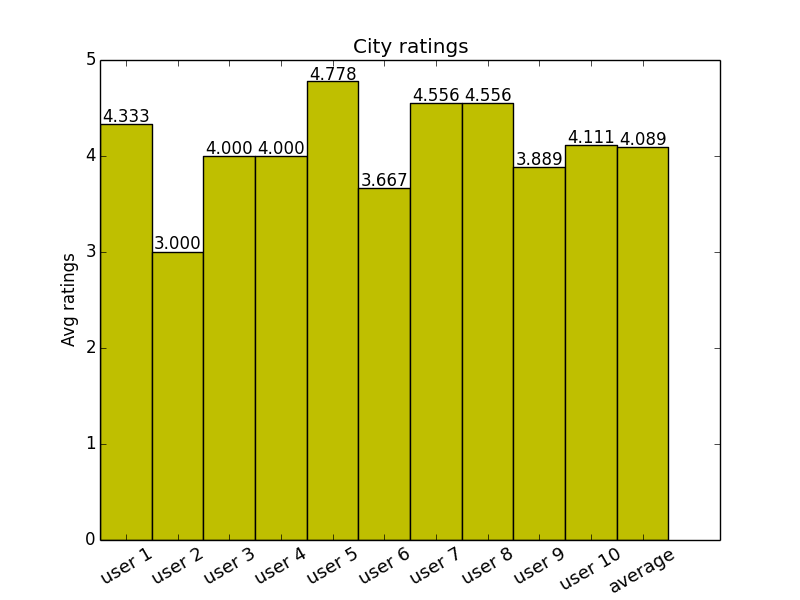
\includegraphics[width=90mm]{images/evaluation/average_city_score.png}
\caption{User average rating for city}
\label{fig:city}
\end{figure}

\begin{figure}[H]
\centering
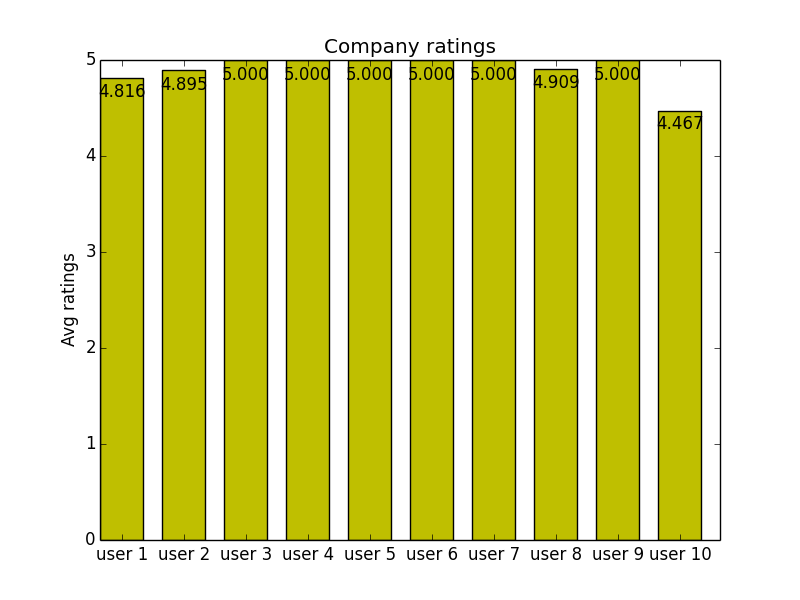
\includegraphics[width=90mm]{images/evaluation/average_company_score.png}
\caption{User average rating for company name}
\label{fig:company}
\end{figure}

\begin{figure}[H]
\centering
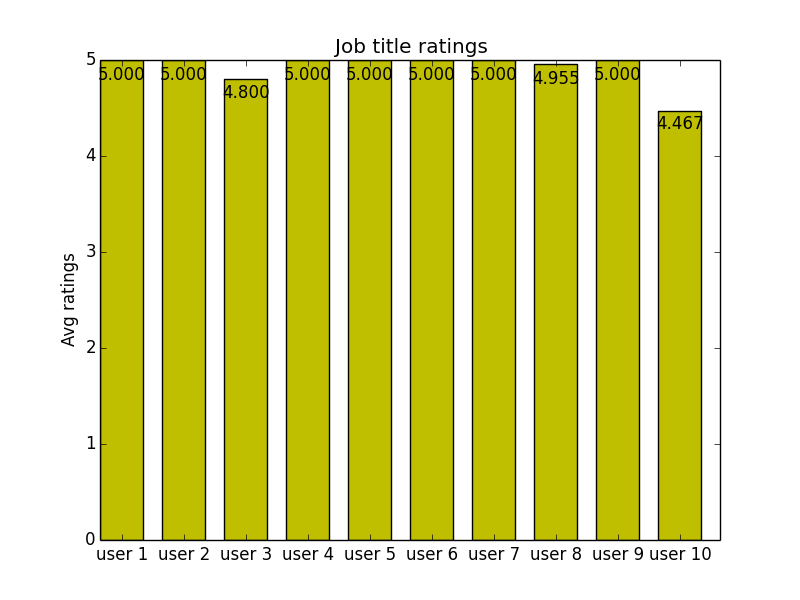
\includegraphics[width=90mm]{images/evaluation/average_job_title_score.png}
\caption{User average rating for job title}
\label{fig:job_title}
\end{figure}

\begin{figure}[H]
\centering
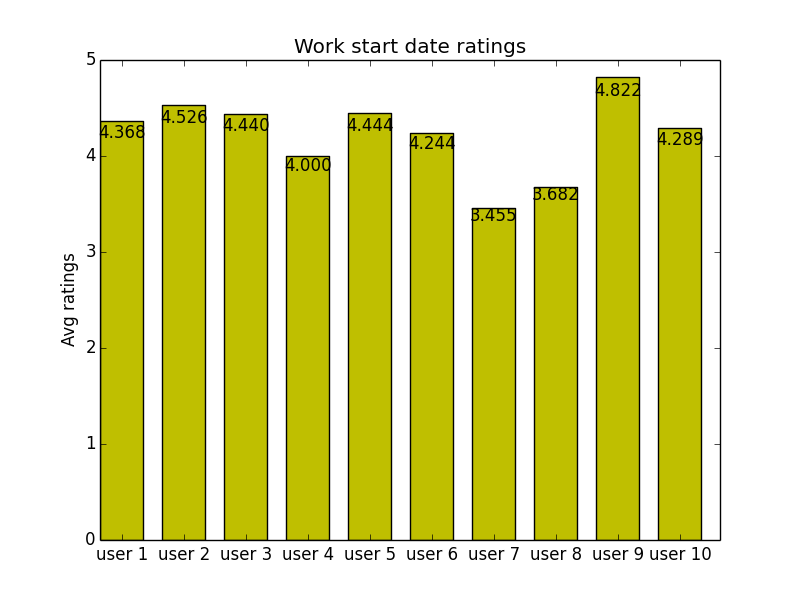
\includegraphics[width=90mm]{images/evaluation/average_experience_start_date_score.png}
\caption{User average rating for experience start data}
\label{fig:experiencestart}
\end{figure}

\begin{figure}[H]
\centering
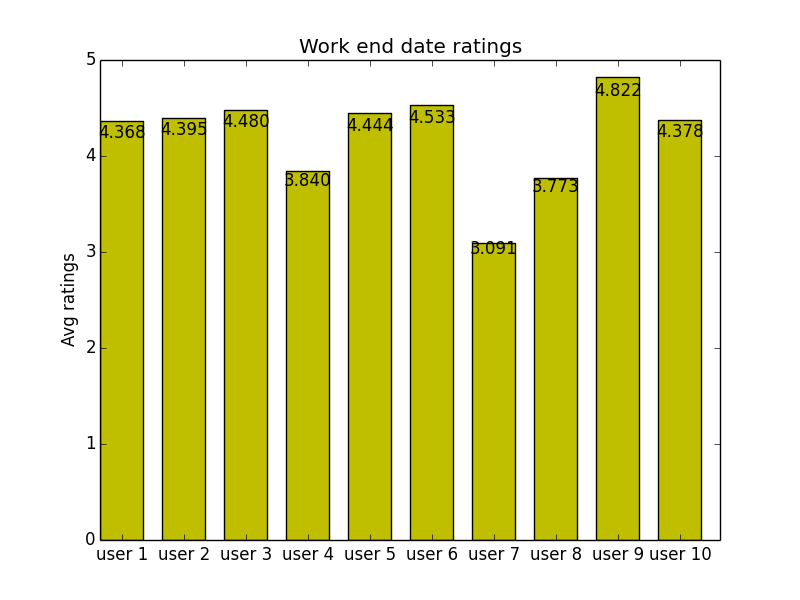
\includegraphics[width=90mm]{images/evaluation/average_experience_end_date_score.png}
\caption{User average rating for experience end data}
\label{fig:experienceend}
\end{figure}

\begin{figure}[H]
\centering
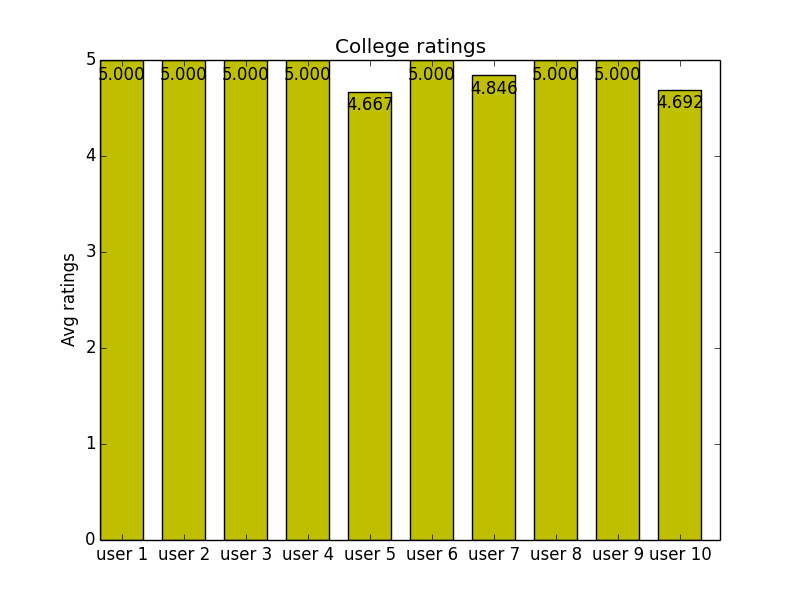
\includegraphics[width=90mm]{images/evaluation/average_college_score.png}
\caption{User average rating for college}
\label{fig:college}
\end{figure}

\begin{figure}[H]
\centering
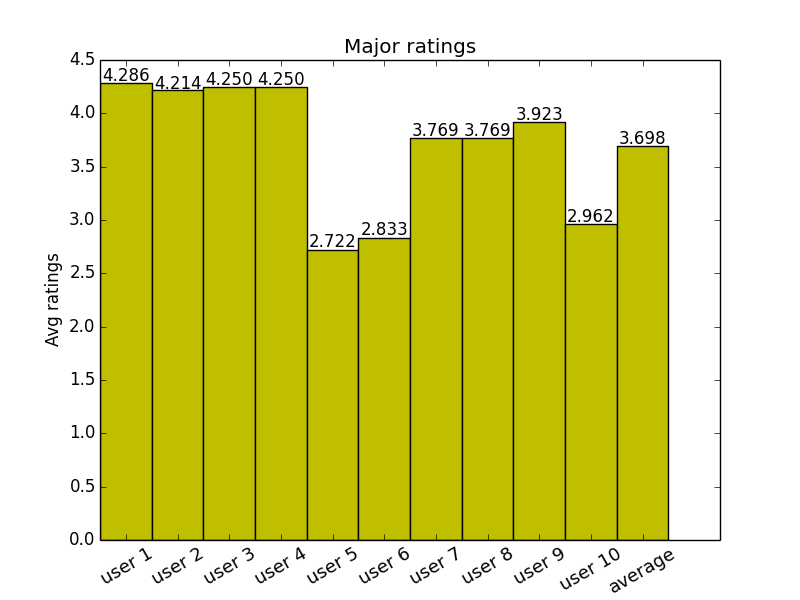
\includegraphics[width=90mm]{images/evaluation/average_major_score.png}
\caption{User average rating for major}
\label{fig:major}
\end{figure}

\begin{figure}[H]
\centering
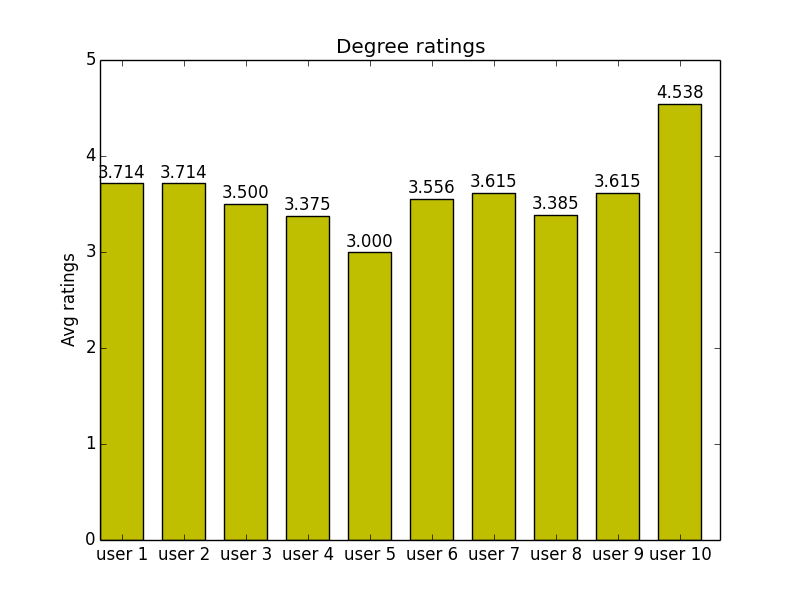
\includegraphics[width=90mm]{images/evaluation/average_degree_score.png}
\caption{User average rating for degree}
\label{fig:degree}
\end{figure}

\begin{figure}[H]
\centering
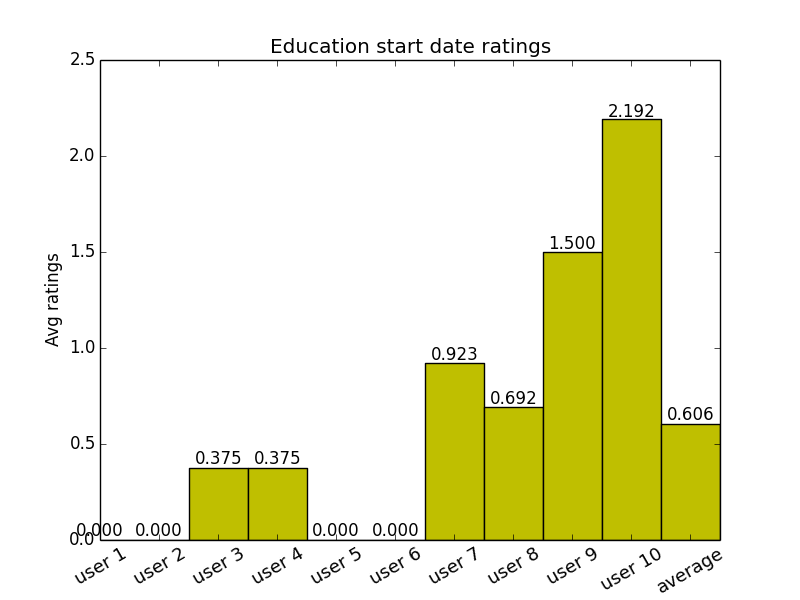
\includegraphics[width=90mm]{images/evaluation/average_education_start_date_score.png}
\caption{User average rating for education start data}
\label{fig:educationstart}
\end{figure}

\begin{figure}[H]
\centering
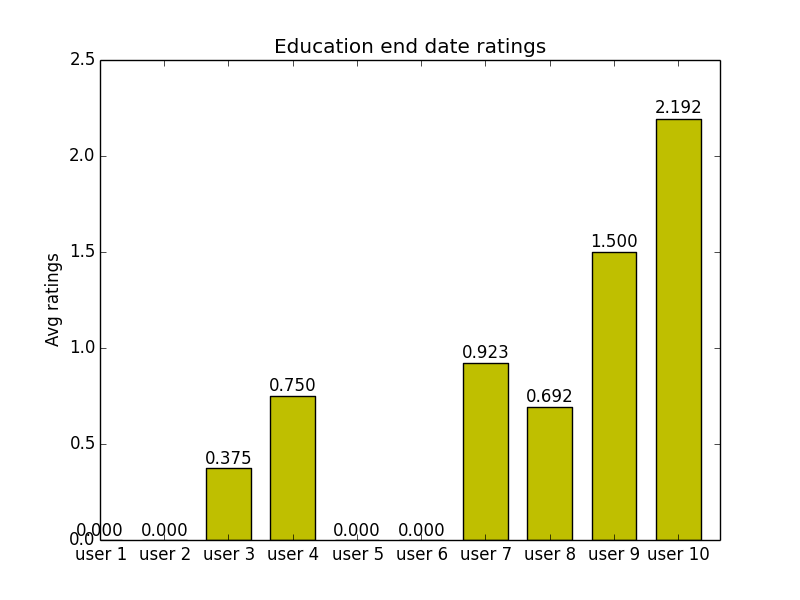
\includegraphics[width=90mm]{images/evaluation/average_education_end_date_score.png}
\caption{User average rating for education end data}
\label{fig:educationend}
\end{figure}

\subsection{Metadata fitness}

This section is a reflection on how the extracted triples fit to the data visualisation interface. The interface is divided into 3 scenarios: 

\begin{description}
	\item Scenario 1, Government \hfill \\
	The first scenario is that the interface should reflect the needs of Government officers. The fields that used by them are: city, industry type, academic degree and company size.
	\item Scenario 2, Company's human resource department \hfill \\
	The user interface also support daily queries from HR. The fields that used in this scenario are: city, degree, skill, work experience and start date.
	\item Scenario3, Job seeker and college student
	This part allows users get insights about the employment status by city. The fields that used in this scenario are: city, degree, skill and position.
\end{description}

During the development and evaluation, we found there're some drawbacks of the extracted data that makes the user interface hard to develop and use:
\begin{enumerate}
	\item Do not have information to group similar job title together.
	\item Colleges, companies may have aliases.
\end{enumerate}

\section{Results}

\subsection{Contributed vocabulary}

\subsection{RDF triples}